\documentclass[]{article}
\usepackage{lmodern}
\usepackage{amssymb,amsmath}
\usepackage{ifxetex,ifluatex}
\usepackage{fixltx2e} % provides \textsubscript
\ifnum 0\ifxetex 1\fi\ifluatex 1\fi=0 % if pdftex
  \usepackage[T1]{fontenc}
  \usepackage[utf8]{inputenc}
\else % if luatex or xelatex
  \ifxetex
    \usepackage{mathspec}
  \else
    \usepackage{fontspec}
  \fi
  \defaultfontfeatures{Ligatures=TeX,Scale=MatchLowercase}
\fi
% use upquote if available, for straight quotes in verbatim environments
\IfFileExists{upquote.sty}{\usepackage{upquote}}{}
% use microtype if available
\IfFileExists{microtype.sty}{%
\usepackage{microtype}
\UseMicrotypeSet[protrusion]{basicmath} % disable protrusion for tt fonts
}{}
\usepackage[margin=1in]{geometry}
\usepackage{hyperref}
\hypersetup{unicode=true,
            pdftitle={February 2019 - Xinavane charts reproduction},
            pdfborder={0 0 0},
            breaklinks=true}
\urlstyle{same}  % don't use monospace font for urls
\usepackage{graphicx,grffile}
\makeatletter
\def\maxwidth{\ifdim\Gin@nat@width>\linewidth\linewidth\else\Gin@nat@width\fi}
\def\maxheight{\ifdim\Gin@nat@height>\textheight\textheight\else\Gin@nat@height\fi}
\makeatother
% Scale images if necessary, so that they will not overflow the page
% margins by default, and it is still possible to overwrite the defaults
% using explicit options in \includegraphics[width, height, ...]{}
\setkeys{Gin}{width=\maxwidth,height=\maxheight,keepaspectratio}
\IfFileExists{parskip.sty}{%
\usepackage{parskip}
}{% else
\setlength{\parindent}{0pt}
\setlength{\parskip}{6pt plus 2pt minus 1pt}
}
\setlength{\emergencystretch}{3em}  % prevent overfull lines
\providecommand{\tightlist}{%
  \setlength{\itemsep}{0pt}\setlength{\parskip}{0pt}}
\setcounter{secnumdepth}{0}
% Redefines (sub)paragraphs to behave more like sections
\ifx\paragraph\undefined\else
\let\oldparagraph\paragraph
\renewcommand{\paragraph}[1]{\oldparagraph{#1}\mbox{}}
\fi
\ifx\subparagraph\undefined\else
\let\oldsubparagraph\subparagraph
\renewcommand{\subparagraph}[1]{\oldsubparagraph{#1}\mbox{}}
\fi

%%% Use protect on footnotes to avoid problems with footnotes in titles
\let\rmarkdownfootnote\footnote%
\def\footnote{\protect\rmarkdownfootnote}

%%% Change title format to be more compact
\usepackage{titling}

% Create subtitle command for use in maketitle
\newcommand{\subtitle}[1]{
  \posttitle{
    \begin{center}\large#1\end{center}
    }
}

\setlength{\droptitle}{-2em}

  \title{February 2019 - Xinavane charts reproduction}
    \pretitle{\vspace{\droptitle}\centering\huge}
  \posttitle{\par}
  \subtitle{Using Maragra data}
  \author{}
    \preauthor{}\postauthor{}
    \date{}
    \predate{}\postdate{}
  
\pagenumbering{gobble}
\usepackage{longtable}
\usepackage[utf8]{inputenc}
\usepackage{changepage}
\usepackage{graphicx}
\usepackage{multicol}
\usepackage{geometry}
\usepackage{fancyhdr}
\usepackage{color}
\usepackage{colortbl}
\usepackage{color}
\usepackage{hyperref}
% Font
\usepackage{fontspec}
\setmainfont{Swift-Regular_43151.ttf}
\setsansfont[BoldFont={Swift-Bold_43130.ttf}]{Swift-Regular_43151.ttf}
% \setmonofont{Swift-Regular_43151.ttf}
\renewcommand{\familydefault}{\sfdefault}
% \usepackage{fontspec}
% \setmainfont{Lato-Regular.ttf}
% \setsansfont[BoldFont={Lato-Bold.ttf}]{Lato-Regular.ttf}
% \renewcommand{\familydefault}{\sfdefault}

\def\changemargin#1#2{\list{}{\rightmargin#2\leftmargin#1}\item[]}
\let\endchangemargin=\endlist
\renewcommand{\rmdefault}{ppl}

\usepackage{multicol}
\usepackage{hyperref}
\usepackage{geometry}
\usepackage{lipsum}

\usepackage{longtable}


\usepackage{float}
\floatplacement{figure}{H}

% \usepackage{todonotes} % for side notes
% \usepackage[colorinlistoftodos]{todonotes} % for side notes

\usepackage{xargs}                      % Use more than one optional parameter in a new commands
\usepackage[dvipsnames, table]{xcolor}  % Coloured text etc.
% 
\usepackage[colorinlistoftodos,prependcaption,textsize=tiny]{todonotes}
\newcommandx{\unsure}[2][1=]{\todo[linecolor=red,backgroundcolor=red!25,bordercolor=red,#1]{#2}}
\newcommandx{\change}[2][1=]{\todo[linecolor=blue,backgroundcolor=blue!25,bordercolor=blue,#1]{#2}}
\newcommandx{\info}[2][1=]{\todo[linecolor=OliveGreen,backgroundcolor=OliveGreen!25,bordercolor=OliveGreen,#1]{#2}}
\newcommandx{\improvement}[2][1=]{\todo[linecolor=Plum,backgroundcolor=Plum!25,bordercolor=Plum,#1]{#2}}
\newcommandx{\thiswillnotshow}[2][1=]{\todo[disable,#1]{#2}}
\usepackage{lmodern}
\usepackage{fancyhdr} % Headers and footers
\pagestyle{fancy} % All pages have headers and footers
\fancyhead{} % Blank out the default header
\fancyfoot{} % Blank out the default footer
\fancyhead[C]{Return on investment of private sector malaria control at a large sugar facility in Southern Mozambique}
\renewcommand{\thefootnote}{\fnsymbol{footnote}}

\newcommand{\footremember}[2]{%
    \footnote{#2}
    \newcounter{#1}
    \setcounter{#1}{\value{footnote}}%
}
\newcommand{\footrecall}[1]{%
    \footnotemark[\value{#1}]%
}

\def\changemargin#1#2{\list{}{\rightmargin#2\leftmargin#1}\item[]}
\let\endchangemargin=\endlist

\widowpenalties 1 150

\makeatletter
\renewcommand\footnotesize{%
   \@setfontsize\footnotesize\@ixpt{11}%
   \abovedisplayskip 8\p@ \@plus2\p@ \@minus4\p@
   \abovedisplayshortskip \z@ \@plus\p@
   \belowdisplayshortskip 4\p@ \@plus2\p@ \@minus2\p@
   \def\@listi{\leftmargin\leftmargini
               \topsep 4\p@ \@plus2\p@ \@minus2\p@
               \parsep 2\p@ \@plus\p@ \@minus\p@
               \itemsep \parsep}%
   \belowdisplayskip \abovedisplayskip
}
\makeatother

\DeclareTextCommandDefault{\nobreakspace}{\leavevmode\nobreak\ }
\usepackage{booktabs}
\usepackage{longtable}
\usepackage{array}
\usepackage{multirow}
\usepackage[table]{xcolor}
\usepackage{wrapfig}
\usepackage{float}
\usepackage{colortbl}
\usepackage{pdflscape}
\usepackage{tabu}
\usepackage{threeparttable}
\usepackage{threeparttablex}
\usepackage[normalem]{ulem}
\usepackage{makecell}

\begin{document}
\maketitle

\begin{center}
\begin{large}

Charts

\end{large}
\end{center}

\vspace{5mm}

\begin{center}
\textbf{Overview}  
\end{center}

\vspace{5mm}

\begin{center}
\begin{changemargin}{3cm}{3cm} 

This document contains charts from Maragra data, meant for comparison with Xinavane. It was created on February 5, 2019 by Joe Brew for Laia Cirera and Elisa Sicuri.

\end{changemargin}
\end{center}

\vspace{20mm}

\noindent\fbox{%
    \parbox{\textwidth}{%
        \subsection*{Action}
        \begin{itemize}
          \item Review charts herein
          \item Request clarification or ask questions if applicable
        \end{itemize}
        \vspace{2mm}
    }%
}

\vfill
\null

\subsection*{Desinataires}

\textbf{Laia Cirera; Elisa Sicuri}

\vspace{3mm}

\newpage

\section{Malaria prevalence in the region, (2013-2017), Manhiça
(control)}\label{malaria-prevalence-in-the-region-2013-2017-manhica-control}

\begin{center}\includegraphics{feb2019_xinavane_reproduction_files/figure-latex/unnamed-chunk-3-1} \end{center}

\section{Malaria prevalence in the region,
(2013-2017)}\label{malaria-prevalence-in-the-region-2013-2017}

Magude (intervention)

\begin{center}\includegraphics{feb2019_xinavane_reproduction_files/figure-latex/unnamed-chunk-4-1} \end{center}

\section{Both locations}\label{both-locations}

\begin{center}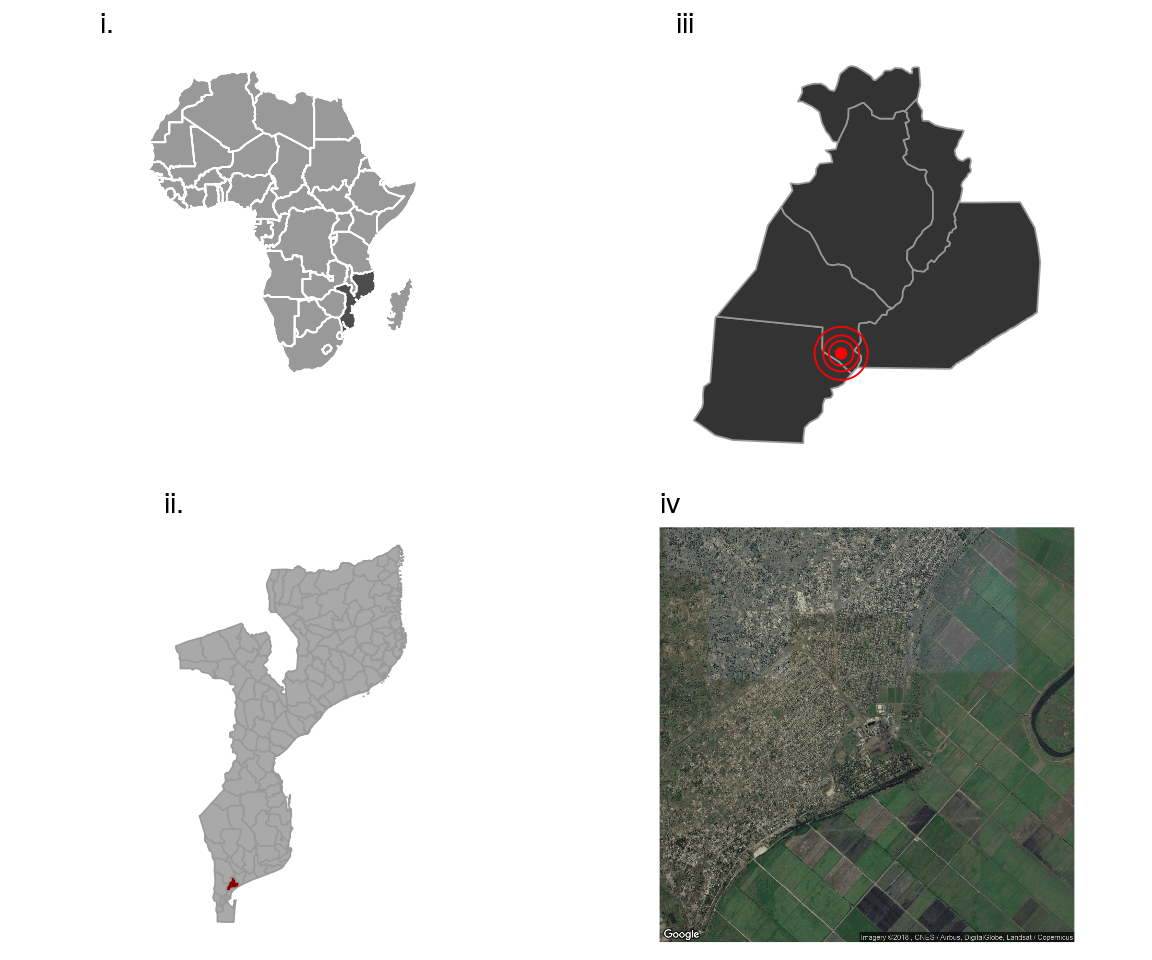
\includegraphics{feb2019_xinavane_reproduction_files/figure-latex/unnamed-chunk-5-1} \end{center}

\subsection{Number of workers by contract
type}\label{number-of-workers-by-contract-type}

\begin{center}\includegraphics{feb2019_xinavane_reproduction_files/figure-latex/unnamed-chunk-6-1} \end{center}

\subsection{Absenteeism rate by contract
type}\label{absenteeism-rate-by-contract-type}

\begin{center}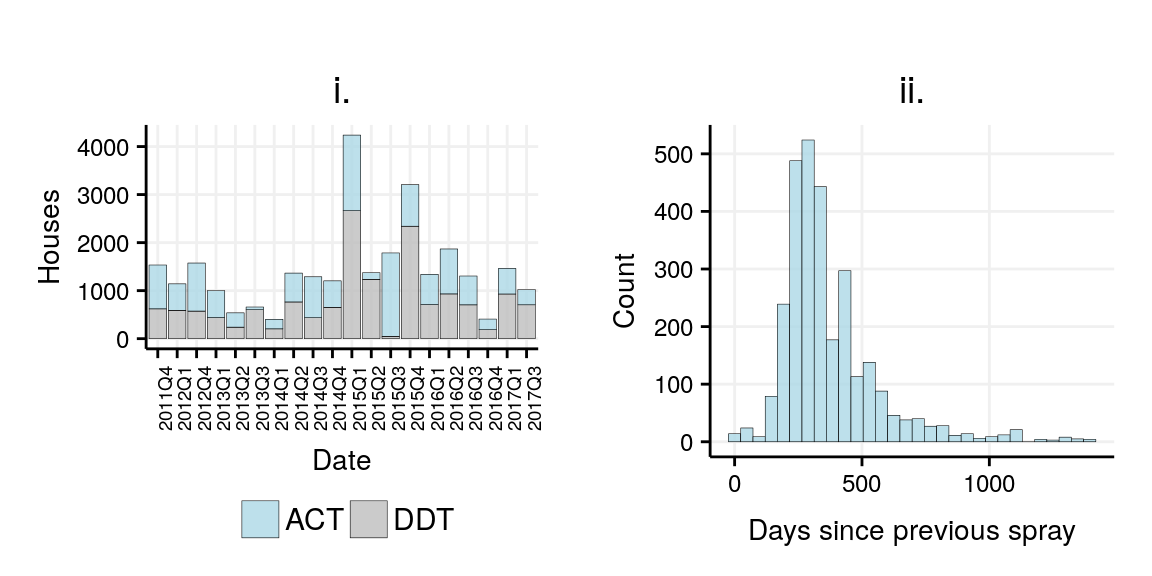
\includegraphics{feb2019_xinavane_reproduction_files/figure-latex/unnamed-chunk-7-1} \end{center}

\subsection{Permanent workers absenteeism rate and malaria
incidence}\label{permanent-workers-absenteeism-rate-and-malaria-incidence}

\begin{center}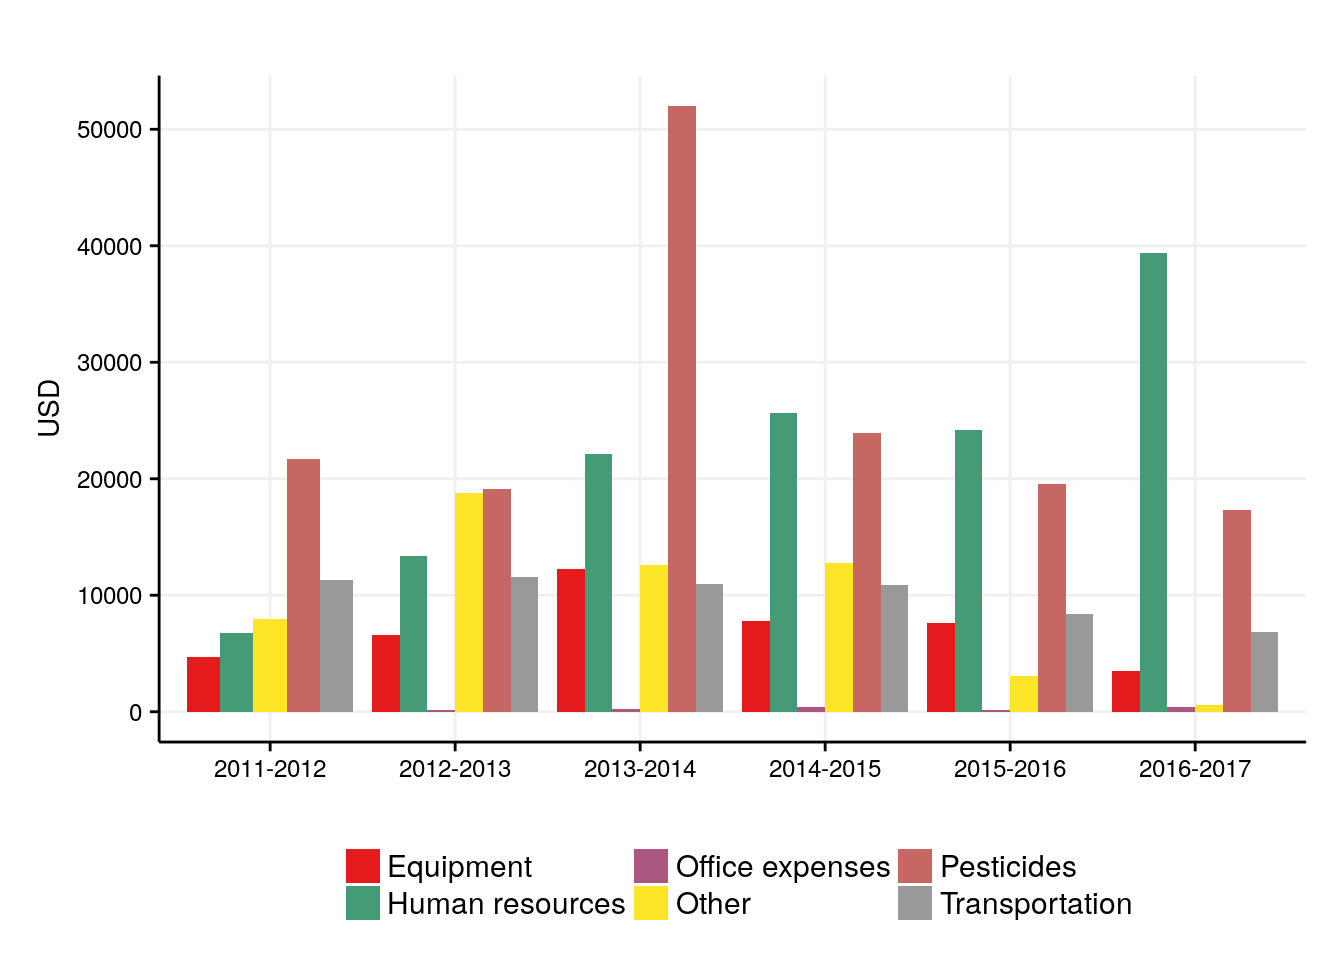
\includegraphics{feb2019_xinavane_reproduction_files/figure-latex/unnamed-chunk-8-1} \end{center}

\subsection{Number of temporary workers by job
type}\label{number-of-temporary-workers-by-job-type}

(Skipped due to category incompatibility)

\subsection{Temporary workers absenteeism rate and malaria
incidence}\label{temporary-workers-absenteeism-rate-and-malaria-incidence}

(Modified due to category incompatability)

\begin{center}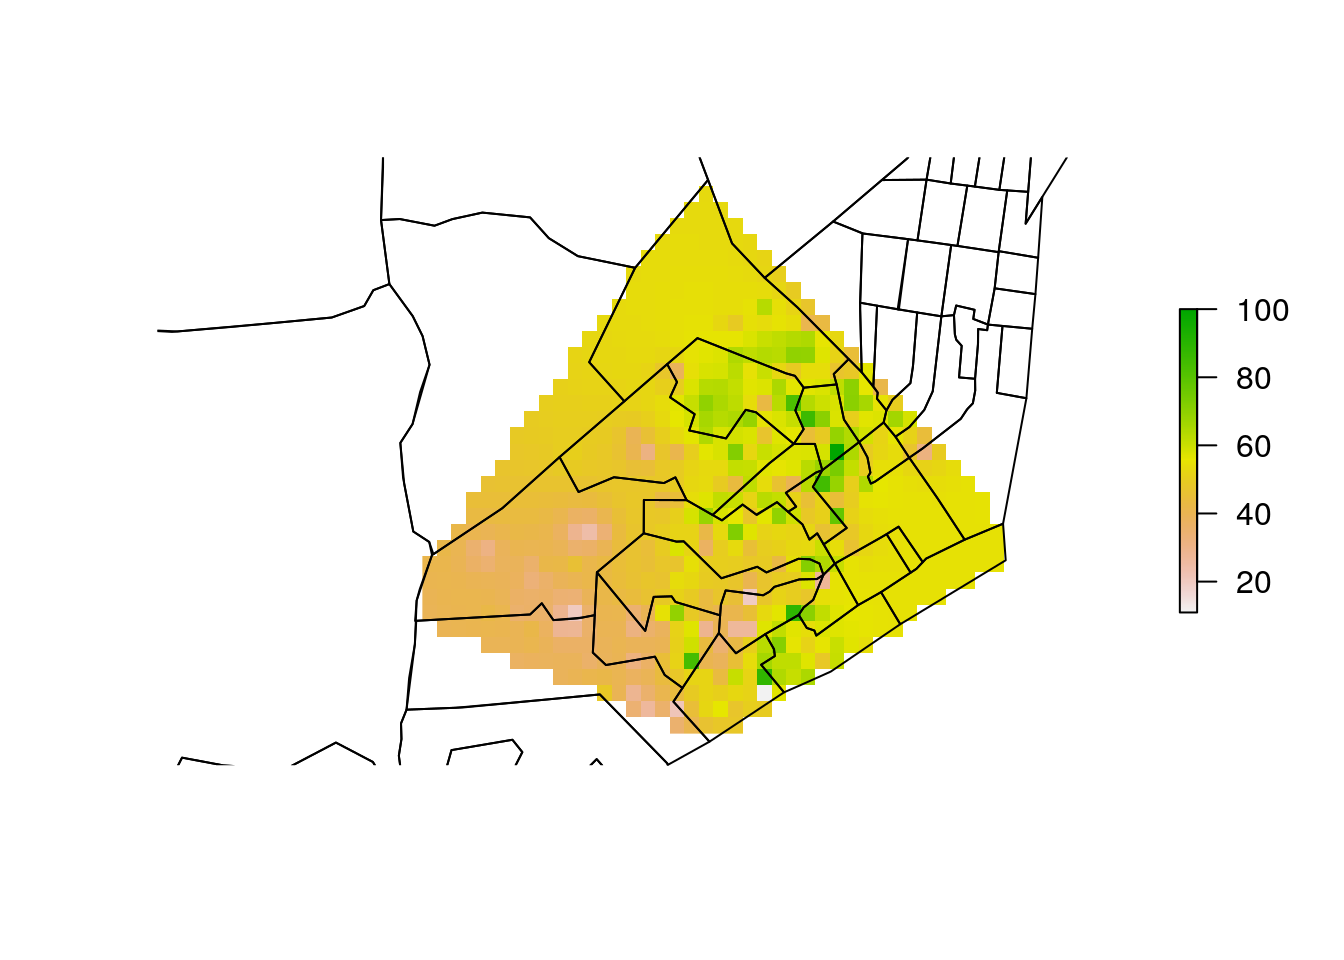
\includegraphics{feb2019_xinavane_reproduction_files/figure-latex/unnamed-chunk-9-1} \end{center}

\newpage

\section{Other miscellaneous charts}\label{other-miscellaneous-charts}

\subsection{Number of workers by
department}\label{number-of-workers-by-department}

\begin{center}\includegraphics{feb2019_xinavane_reproduction_files/figure-latex/unnamed-chunk-10-1} \end{center}

\subsection{Number of temporary workers over
time}\label{number-of-temporary-workers-over-time}

\begin{center}\includegraphics{feb2019_xinavane_reproduction_files/figure-latex/unnamed-chunk-11-1} \end{center}

\subsection{Absenteeism rate over
time}\label{absenteeism-rate-over-time}

\begin{center}\includegraphics{feb2019_xinavane_reproduction_files/figure-latex/unnamed-chunk-12-1} \end{center}

\subsection{Absenteeism rate over time by worker
type}\label{absenteeism-rate-over-time-by-worker-type}

\begin{center}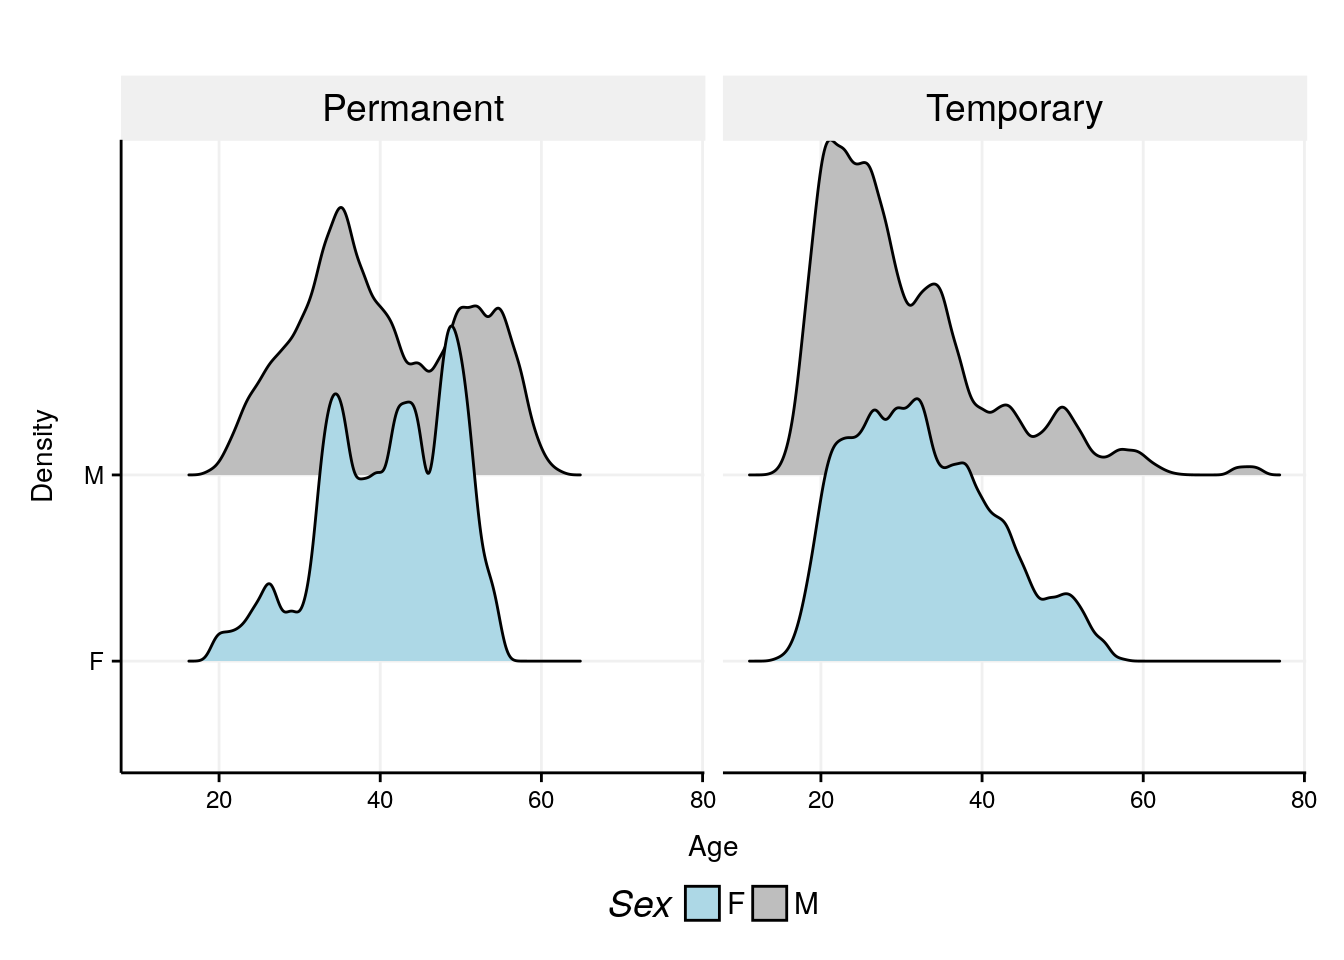
\includegraphics{feb2019_xinavane_reproduction_files/figure-latex/unnamed-chunk-13-1} \end{center}

\subsection{Number of workers over time by worker
type}\label{number-of-workers-over-time-by-worker-type}

\begin{center}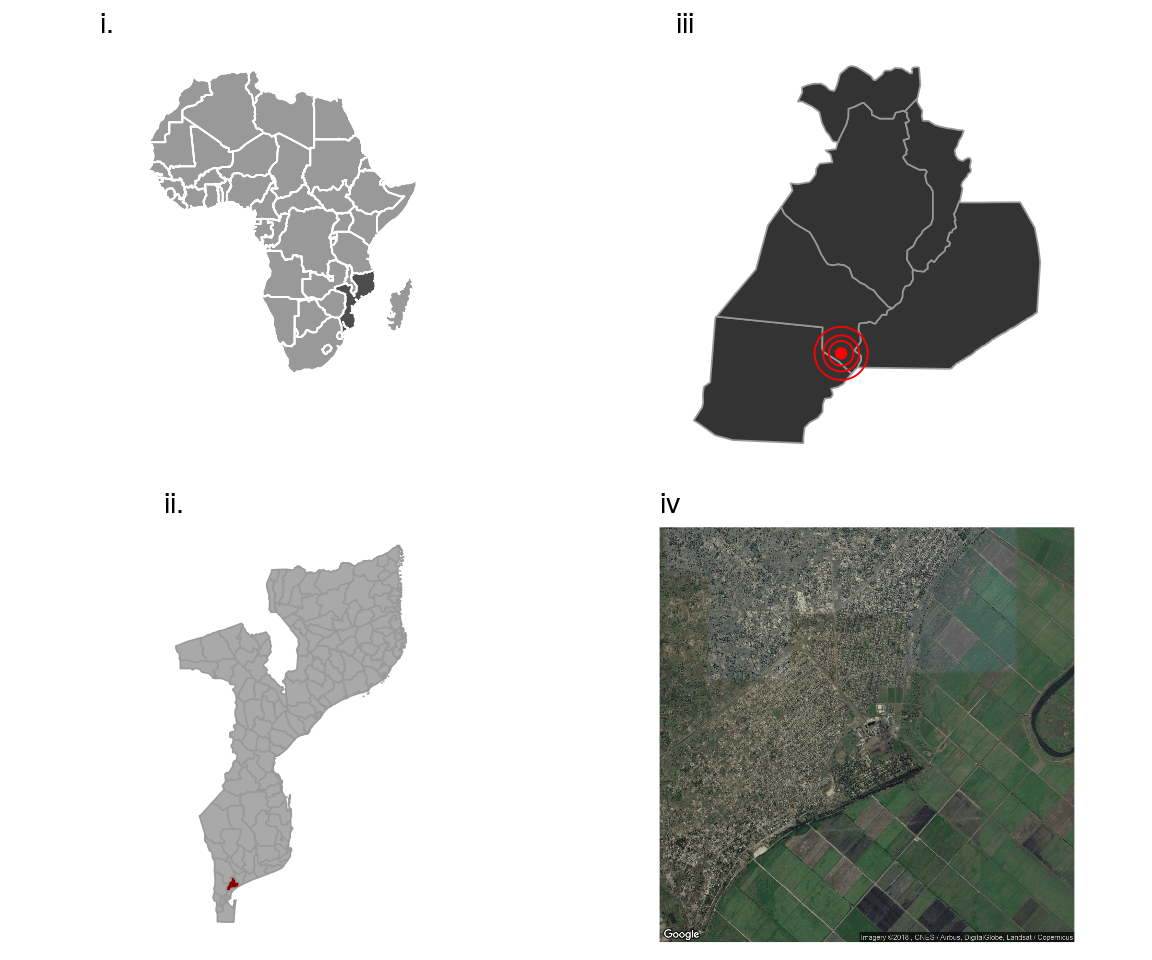
\includegraphics{feb2019_xinavane_reproduction_files/figure-latex/unnamed-chunk-14-1} \end{center}

\section{Bibliography}\label{bibliography}


\end{document}
